% Created 2022-05-14 Сб 14:28
% Intended LaTeX compiler: xelatex
\documentclass[11pt]{article}
\usepackage{graphicx}
\usepackage{longtable}
\usepackage{wrapfig}
\usepackage{rotating}
\usepackage[normalem]{ulem}
\usepackage{amsmath}
\usepackage{amssymb}
\usepackage{capt-of}
\usepackage{hyperref}
\usepackage[utf8x]{inputenc}
% \usepackage[T2A]{fontenc}

\usepackage[russian, english]{babel}
\babelfont{rm}{Droid Serif}
\babelfont{sf}{Droid Sans}
\babelfont{tt}{Droid Sans Mono Slashed}

\hypersetup{colorlinks=true,linkcolor=blue}

\let\oldsection\section
\renewcommand\section{\pagebreak\oldsection}

\usepackage{siunitx}
\sisetup{per-mode=symbol}

% \usepackage{minted}

\author{Андрей Люнгрин Иван Наумов}
\date{11 Мая 2022}
\title{Инженеры будущего\\\medskip
\large Rescue line}
\hypersetup{
 pdfauthor={Андрей Люнгрин Иван Наумов},
 pdftitle={Инженеры будущего},
 pdfkeywords={},
 pdfsubject={},
 pdfcreator={Emacs 28.1 (Org mode 9.6)}, 
 pdflang={English}}
\begin{document}

\maketitle
\tableofcontents


\section{Введение}
\label{sec:org6421151}
Наша работа представляет из себя исследовательский проект проводимый в рамках соревнований под регламентов \texttt{RoboCup Junior RescueLine}. В рамках данной работы нами было разработано несколько прототипов роботизированных систем о которых пойдёт речь далее.
\section{Команда}
\label{sec:org86729b5}
\subsection{Андрей Люнгрин}
\label{sec:org38e4e5d}
\begin{center}
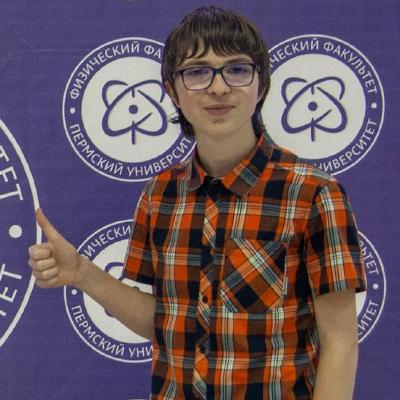
\includegraphics[width=100]{./images/andrey.jpeg}
\end{center}
\begin{itemize}
\item Капитан команды
\item Обязанности:
\begin{itemize}
\item Консультация по вопросам конструкции
\item Производство некоторых деталей
\item Финальная сборка и тестирование конструкции
\item Проектирование концепта
\item Разработка программных компонентов низкого уровня для управления приводами
\item Разработка программных компонентов для обеспечения связи между системами управления приводами и принятия решений
\item Разработка программной системы принятия решений
\item Сборка электронной составляющей робота
\item И просто хороший человек
\end{itemize}
\end{itemize}
\pagebreak
\subsection{Иван Наумов}
\label{sec:orgd69d41a}
\begin{center}
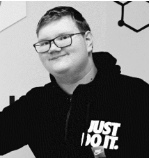
\includegraphics[width=100]{./images/ivan.jpg}
\end{center}
\begin{itemize}
\item Инженер-конструктор
\item Обязанности:
\begin{itemize}
\item Проектирование концепта
\item Моделирование конструкции робота в САПР
\item Производство основных деталей конструкци
\item Сборка конструкции
\end{itemize}
\end{itemize}
\section{Механическая часть}
\label{sec:org232a892}
Основными целями при проектированнии конструкции были простоата и удобство обслуживания, и все последующие технические решения были направлены на улучшение этих двух метрик.

Все узлы робота были произведены с исопльзованием трёхмерной печати

\begin{center}
\includegraphics[width=.9\linewidth]{./images/hw-1.png}
\end{center}
\begin{center}
\includegraphics[width=.9\linewidth]{./images/hw-2.png}
\end{center}

\subsection{Колёсная платформа}
\label{sec:orgbaa6b48}
Конструктивно, робот представляет их себя четырёхколёсную тележку с двумя ведущими и двумя опорными колёмами. Опорные колеса были модифицированы так, чтобы максимально уменьшить сцепление с поверхностью. Это необходимо для того, чтобы кинематическая схема робота была приближена к таковой у двухколесного робота. Плюс такой схемы заключается в том, что ось поворота робота более предсказуема, и в меньшей степени зависит от распределения массы.

Каждое колесо имеет две точки опоры, что позволяет снизить изламывающие нагрузки на ось колеса, что увеличивает надёжность конструкции, а также делает положение колеса относительно рамы робота более предсказуемым.
\pagebreak
\subsection{Система захвата}
\label{sec:org87258b6}
Для захвата и сброса шариков и других игровых предметов, используется двух-осевой манипулятор. Первая ось обеспечивет подъём за счёт поворота всей сборки захвата. Вторая ось является клешнёй, которая выполняет захват объекта. Основное достоинство такой конструкции - её просто. Из недостатков, можно отметить её низкую точность позиционирования, и необходимость приложения высокого усилия мотором подъёма.
\subsection{Крепление электроники}
\label{sec:org4eafc83}
Вся электронника робота закреплена на одной съёмной пластине, расположенной перпендикулярно плоскости рамы. Две основных платы раположены с разных сторон пластины. Такая конфигурация обеспечивает полный доступ ко всем элементам системы, а также позволяет быстро их демонтировать для замены или другого обслуживания.
\section{Электронная часть}
\label{sec:org6770896}
Наша система состоит из трёх основных узлов:
\begin{enumerate}
\item Узел питания
\begin{itemize}
\item Распределяет питание из одного источника между всеми потребителями
\item Согласовывает питающие уровни
\item Состоит из:
\begin{itemize}
\item Высокотоковый литий-полимерный аккумулятор на 12V
\item Понижающий преобразователь
\item Соединительные колодки \texttt{Wago}
\end{itemize}
\end{itemize}
\item Узел принятия решений
\begin{itemize}
\item Получает и обрабатывает информацию об окружающем мире
\item Состоит из:
\begin{itemize}
\item Одноплатный компьютер: \texttt{Raspberry Pi 3B}
\item Основная передняя камера, для следования по линии: \texttt{Pi Camera}
\item Задняя камера для захвата предметов
\end{itemize}
\end{itemize}
\item Исполнительный узел
\begin{itemize}
\item Управляет шаговыми двигателями в ответ на команды с Узла принятия решений
\item Состоит из:
\begin{itemize}
\item Микроконтроллер на отладочной плате: \texttt{STN32 Nucleo-F401RE}
\item Материнская плата драйверов ШД: \texttt{Arduino CNC shield v3}
\item Четыре драйвера ШД: \texttt{StepStick A4988}
\item Два приводных шаговых двигателя
\item Два шаговых двигателя для манипулятора
\end{itemize}
\end{itemize}
\end{enumerate}

Шаговые двигатели для привода были использованы потому, что такой тип двигателя позволяет просто контроллировать их скорость, также тем, что существует множество готовых аппаратных решений для их управления. Простота управления и цена - вероятно единственные приимещества шаговых двигателей. К их недостаткам относятся: низкий КПД, низкое соотношение крутящего к массе двигателя, сильные вибрации. К счастью, все эти приблемы не значительны в нашем случае (нету ограничения по весу, низкие требования к тяге и времени автономной работы, а критерий простоты управления хорошо соотносится с целями проекта.

Решение использовать отдельный контроллер для управления двигателями были обосновано тем, что реализовать генерацию управляющих пульсов для драйверов ШД с микросекундной точностью, проще на системе реального времени, работая на низком уровне. Однако, такой подход влечет за собой усложнение системы, из-за необходимости обеспечивать связь между двумя контроллерами. В будущем, второй контроллер может быть упразднён.

\begin{center}
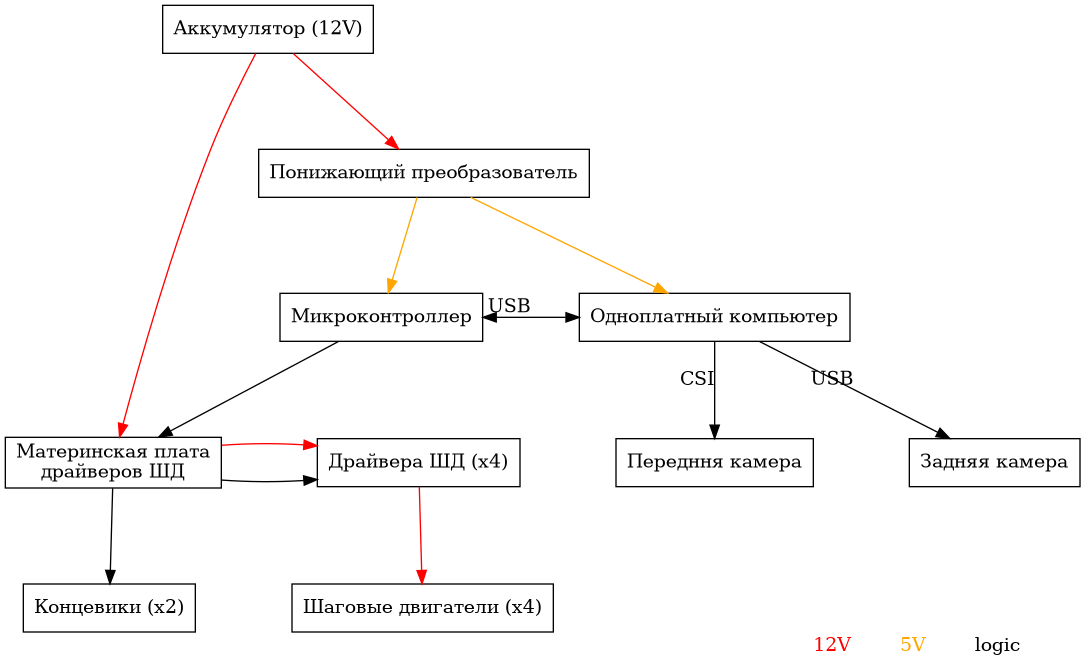
\includegraphics[width=.9\linewidth]{images/electronics-diag.png}
\end{center}
\section{Программная часть}
\label{sec:orgcaf9a01}
Разработка ПО велась с исопльзованием системы контроля версий \texttt{Git}. Весь код открыт и доступен на GitHub по ссылке \url{https://github.com/prostoiChelovek/rescue-line-2022}
\subsection{Контроллер двигателей}
\label{sec:org568d73d}
Программа для микроконтраллера была написана на \texttt{Rust} с использованием фреймворка \texttt{RTIC}. \texttt{Rust} - компилируемый, статически типизированный язык программирования среднего уровня, основной особенностью которого является гарантия безопасности управления памяти на этапе компиляции. \texttt{RTIC} - Real Time Interrupt-driven Concurency - библиотека реализующая конкурентность, удобный интерфейс для управления общими ресурсами, а также гарантию отсутствия взаимных блокировок на этапе компиляции.

Генерация управляющего сигнала для драйверов ШД реализована с исопльзованием планировщика задач \texttt{RTIC}. Структура, представляющая шаговый двигатель, предоставляет метод \texttt{update}, который обновляет внутреннее состояние структуры, и может обновить уровень на выходе контроллера. Метод возвращает время, через которое он должен быть вызван в следующий раз. Внутреннее состояние контроллера ШД представляет из себя машину состояний, которая описывается следующим образом:
\begin{verbatim}
state_machine! {
    Idle(Start) => StartStepHigh, // Состояние_1(Событие) => Состояние_2

    StartStepHigh(PulseStart) => StepHigh,
    StepHigh(PulseEnd) => StartStepLow,

    StartStepLow(PulseStart) => StepLow,
    StepLow(PulseEnd) => StartStepHigh,

    Idle(Stop) => Idle,
    StartStepHigh(Stop) => Idle,
    StepHigh(Stop) => StartStepLow [Stop],
    StartStepLow(Stop) => Idle,
    StepLow(Stop) => Idle,
}
\end{verbatim}

Сам метод выглядит следующим образом:
\begin{verbatim}
pub fn update(&mut self) -> Option<MicrosDurationU32> {
    if self.step_delay.is_none() {
        return None;
    }

    match *self.state_machine.state() {
        StepperStateState::Idle => { None }
        StepperStateState::StartStepHigh => {
            self.step.set_high().ok();
            self.state_machine.consume(
                        &StepperStateInput::PulseStart).unwrap();

            Some(self.pulse_width)
        },
        StepperStateState::StartStepLow => {
            self.step.set_low().ok();
            self.state_machine.consume(
                        &StepperStateInput::PulseStart).unwrap();

            Some(self.step_delay.unwrap())
        },
        StepperStateState::StepHigh | StepperStateState::StepLow => {
            self.state_machine.consume(
                        &StepperStateInput::PulseEnd).unwrap();

            self.update()
        }
    }
}
\end{verbatim}

Такой дизайн обусловлен тем, что, этот метод вызывается часто (до 5кГц), и имеет приоритет выше других задач, т.е. может прервать их выполнение. Проблема становится более заметной, если учесть, что одновременно могут работать до четырёх двигателей.

Использование этого модуля в программе выгладит так:
\begin{verbatim}
#[init]
fn init(mut ctx: init::Context) -> (Shared, Local, init::Monotonics) {
    let rcc = ctx.device.RCC.constrain();
    let clocks = rcc.cfgr.sysclk(84.mhz()).freeze();
    let mut syscfg = ctx.device.SYSCFG.constrain();

    let gpiob = ctx.device.GPIOB.split();

    let right_stepper = {
        let (step, dir) = (gpiob.pb3.into_push_pull_output(),
                           gpiob.pb10.into_push_pull_output());
        let mut stepper = Stepper::new(step, dir,
                                       || right::spawn().unwrap());
        stepper.set_direciton(StepperDireciton::CounterClockwise);
        stepper.set_speed(100_u32.Hz());
        stepper
    };

    (
        Shared { right_stepper },
        Local { },
        init::Monotonics(mono)
    )
}

#[task(shared = [right_stepper], priority = 15)]
fn right(mut cx: right::Context) {
    cx.shared.right_stepper.lock(|stepper| {
        let next_delay = stepper.update();
        if let Some(next_delay) = next_delay {
            right::spawn_after(next_delay).ok();
        }
    });
}
\end{verbatim}
\subsection{Протокол взаимодействия}
\label{sec:org002bfc1}
Для синхронизации двух контроллеров используется просто RPC фреймворк, написанный на расте. Основная особенность архитектуры этого модуля в том, что обе стороны исопльзуют одинаковый код, что существенно упрощает поддержку системы, внесение модификаций а также предотвращает ошибки.
Каждое сообщение представляет из себя структура следующего вида:
\begin{verbatim}
#[derive(Clone, Copy, Encode, Decode, PartialEq, Debug)]
pub enum Command {
    Stop,
    SetSpeed(SetSpeedParams),
    OpenGripper,
    CloseGripper,
    LiftGripper,
    LowerGripper
}

#[derive(Clone, Copy, Encode, Decode, PartialEq, Debug)]
pub struct SetSpeedParams {
    pub left: i32,
    pub right: i32
}

#[derive(Encode, Decode, PartialEq, Debug)]
pub enum Message {
    Command(IdType, Command),
    Ack(IdType),
    Done(IdType),
}
\end{verbatim}
Благодаря возможностям языка Rust и исопльзованный библитеки, всё, сериализация и десериализация сообщений реализуюется в одну строку.
\subsection{Зрение}
\label{sec:orgeee9851}
Распознавание линий было реализовано с использованием библиотеки компьютерного зрения \texttt{OpenCV} на \texttt{Python 3}.

Был выбран простейший из эффективных алгоритм: изображение сегментируется по цвету, а после - линия определяется по двум точкам. Каждая точка (её координата \texttt{X}) находится с помощью скользящего окна. Код, ответственный за этого выглядит так:
\begin{verbatim}
def validate_window(win: Union[cv.Mat, Window]) -> bool:
    if isinstance(win, Window):
        win = win.roi
    return all([
        not is_mat_empty(lower_row(win)),
        not is_mat_empty(upper_row(win)),
        get_fill_frac(win) < 0.2,
        ])


def find_window(img: cv.Mat,
                start: float = 0,
                max_offset: Optional[float] = None,
                step: Optional[float] = None) -> Optional[Window]:
    max_offset  = max_offset or windows_in_image(img)
    step = step or 1.0

    for pos in arange_offset(start, max_offset, step, include_end=True):
        win = Window(img, pos)
        if validate_window(win):
            return win
    return None
\end{verbatim}
После того, как были найдены два окна, в них нужно найти соответствующие регионы (их может быть несколько из-за шума). Это происходит следующим образом:
\begin{verbatim}
def get_best_region(regions: List[RegionProperties]) -> RegionProperties:
    # prefers bigger regions closer to left
    return max(regions,
               key=lambda r: 1 / math.sqrt(r.area) + 1 / r.centroid[1])


def reduce_region(region: RegionProperties) -> int:
    return round(region.centroid[1])


def region_width(reg: RegionProperties) -> int:
    start_x, end_x = reg.bbox[1], reg.bbox[3]
    return end_x - start_x


def bound_middle(bound: Tuple[int, int]) -> int:
    return bound[0] + (bound[1] - bound[0]) // 2


def bounds_distance(a: Tuple[int, int], b: Tuple[int, int]) -> int:
    return min(map(abs,
                   (
                   a[1] - b[0],
                   a[0] - b[0],
                   a[1] - b[1],
                   a[0] - b[1],
                   bound_middle(a) - bound_middle(b),
                   )))


def regions_distance(a: RegionProperties, b: RegionProperties) -> int:
    bound_a, bound_b = (a.bbox[1], a.bbox[3]), (b.bbox[1], b.bbox[3])
    return bounds_distance(bound_a, bound_b)


def get_matching_regions(wins: WindowPair) -> List[int]:
    if wins.lower is None and wins.upper is None:
        return []
    elif wins.lower is not None and wins.upper is None:
        return [reduce_region(get_best_region(wins.lower.regions))]
    elif wins.lower is not None and wins.upper is not None:
        lower_regions = wins.lower.regions[:]
        while len(lower_regions) > 0:
            lower_region = get_best_region(lower_regions)

            upper_regions = wins.upper.regions[:]
            while len(upper_regions) > 0:
                upper_region = get_best_region(upper_regions)
                distance = regions_distance(lower_region, upper_region)
                if distance < MAX_REGIONS_DISTANCE:
                    return list(map(reduce_region, (lower_region, upper_region)))
                else:
                    upper_regions.remove(upper_region)
            else:
                lower_regions.remove(lower_region)
        else:  # no matches found
            return [reduce_region(get_best_region(wins.lower.regions))]
\end{verbatim}
Конечным шагом является извлечение информации об отклонении линии от центра и её угле наклона.
\begin{verbatim}
def locate_line(wins: WindowPair) -> LineInfo:
    if wins.lower is None and wins.upper is None:
        raise ValueError("Both windows are empty")

    regions_x = get_matching_regions(wins)
    if len(regions_x) == 0:
        raise ValueError("No matching reigons found")

    img_width = wins.lower.img.shape[1]
    x_offset = regions_x[0] - img_width // 2

    angle = None
    if len(regions_x) == 2:
        x_distance = regions_x[1] - regions_x[0]
        y_distance = wins.lower.start - wins.upper.end
        angle = math.atan(x_distance / y_distance)

    return LineInfo(x_offset, angle)
\end{verbatim}
\begin{center}
\includegraphics[width=.9\linewidth]{./images/vis.png}
\end{center}
\end{document}
